\documentclass[11pt]{article}

%%%%%%%%%%%%%%Include Packages%%%%%%%%%%%%%%%%%%%%%%%%%%
\usepackage{xcolor}
\usepackage{mathtools}
\usepackage[a4paper, total={6in, 8in}, margin=1.25in]{geometry}
\usepackage{amsmath}
\usepackage{amssymb}
\usepackage{paralist}
\usepackage{rsfso}
\usepackage{amsthm}
\usepackage{wasysym}
\usepackage[inline]{enumitem}   
\usepackage{hyperref}
\usepackage{tocloft}
\usepackage{titlesec}
\usepackage{colortbl}
\usepackage{wrapfig}
\usepackage{pdfpages}
\usepackage[american]{circuitikz}
%%%%%%%%%%%%%%%%%%%%%%%%%%%%%%%%%%%%%%%%%%%%%%%%%%%%%%%%



\begin{document}
\Large \noindent \textbf{Physics 5C Discussion (Worksheet 9)}\\
\normalsize
Department of Physics and Astronomy, UCLA\\

\noindent TA: Jinyan Miao (jnmiu@ucla.edu)\\
Office hours: Thursday 2:30 - 4:30 PM (PST) over Zoom \\
Zoom ID: 963 5916 9873 (passcode: hiJinyan)\\
Click for the \href{https://ucla.zoom.us/j/96359169873?pwd=05p7ssCPwTbl8KfxoBNCOuaIbt68jW.1}{\underline{Zoom link}} and \href{https://sites.google.com/umich.edu/jmiu/worksheets}{\underline{solutions to the worksheets}}.\\
\noindent\rule{8cm}{0.4pt}\\

\noindent\textbf{Problem 1}: Changing magnetic flux produces a current.\\

\begin{wrapfigure}[8]{r}{0.6\textwidth}
  \begin{center}
  \vspace{-29pt}
    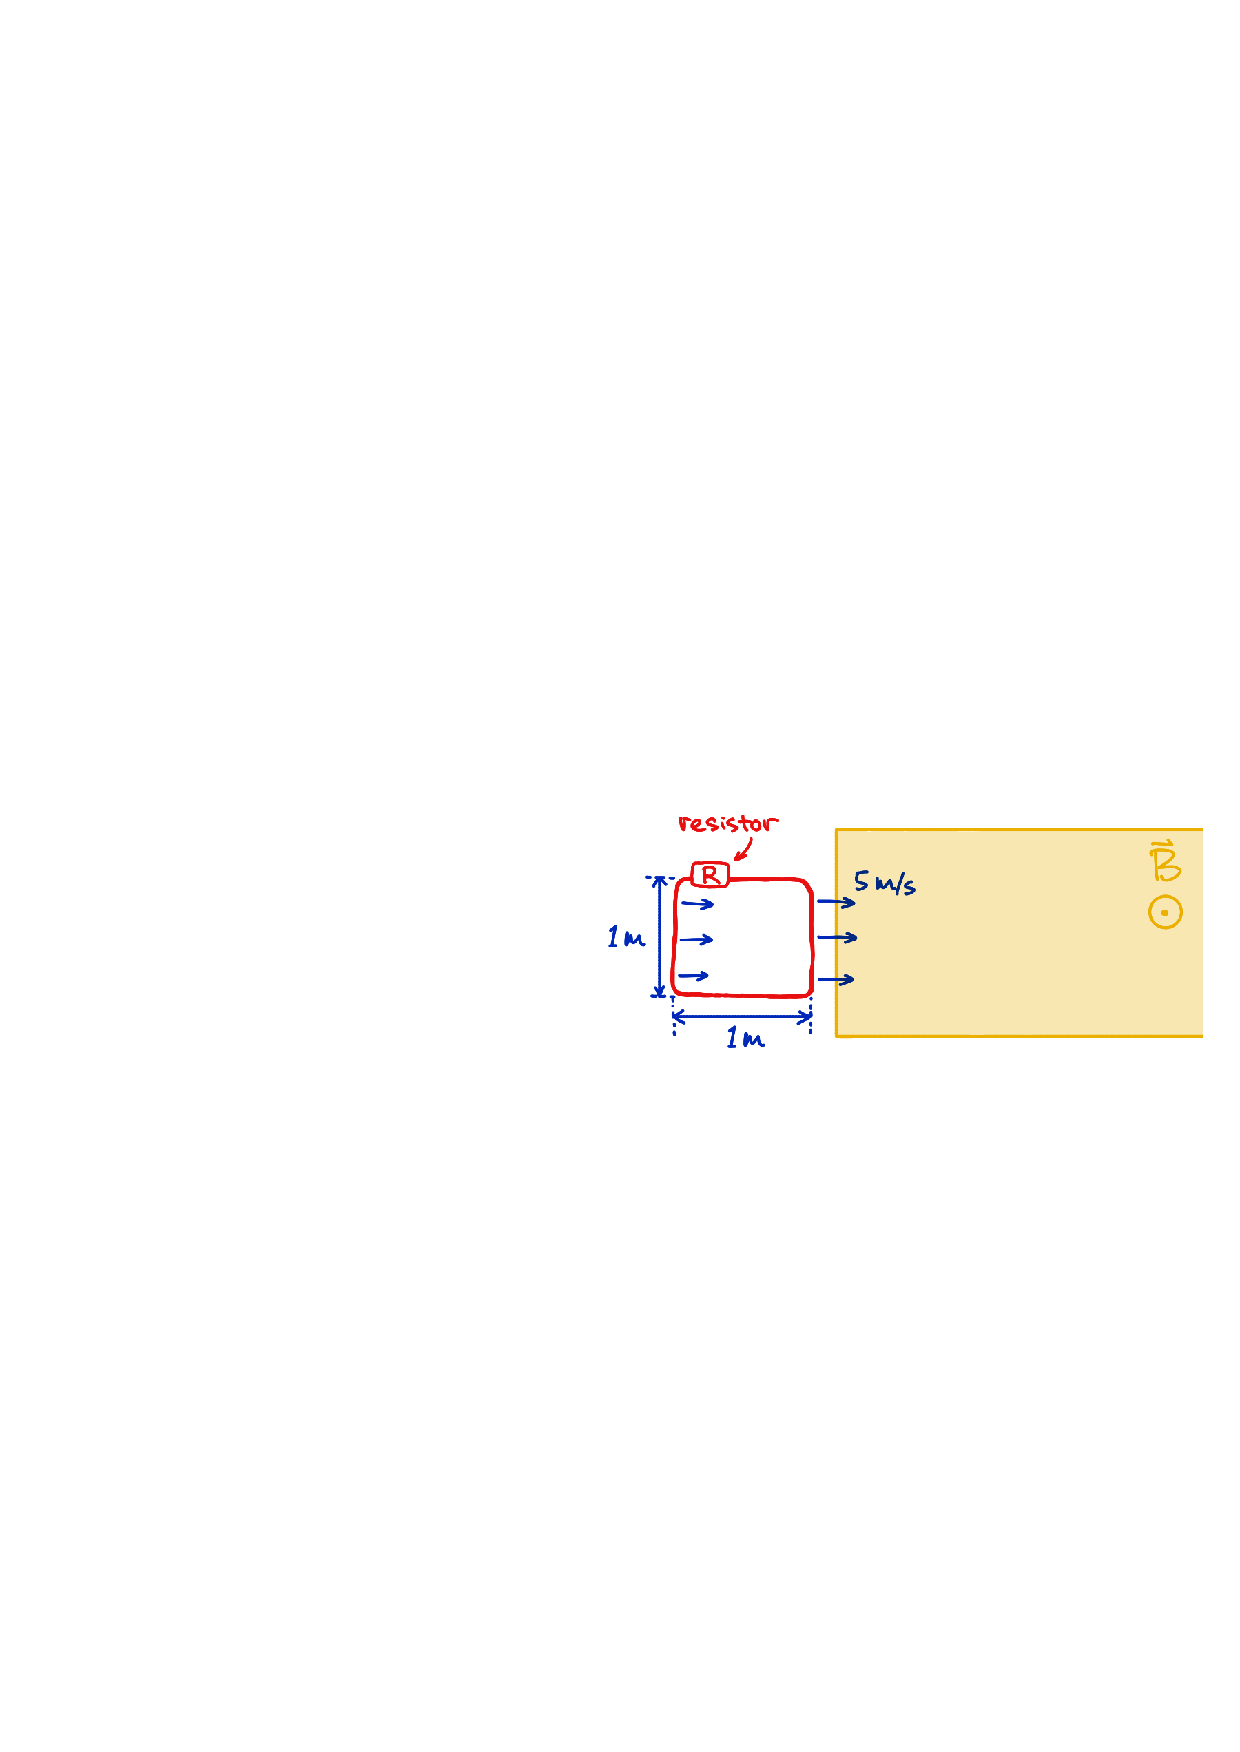
\includegraphics[scale=0.85]{loopInduction}
  \end{center}
\end{wrapfigure}
\noindent Jinyan is moving a square-shaped wire loop into a region (call it region $M$) that has a uniform magnetic field $B = 1\,\text{T}$ in a direction out of the page. The wire loop is moved to the right at a constant speed $5\,$m/s, and the right end of it enters region $M$ at time $t = 0$\,s.\\

\noindent\textbf{Part (a)} Find the area $A$ of the loop that is immersed in region $M$ at an arbitrary time $t>0$. Keep your final answer in terms of $t$.\\

\noindent\textbf{Part (b)} Find the magnetic flux going through the wire loop at arbitrary time $t>0$.\\

\noindent\textbf{Part (c)} When does the magnetic flux through the loop stop changing?\\

\noindent\textbf{Part (d)} Take $R= 5\,\Omega$. At time $t = 0.1$\,s, find the induced emf $\varepsilon$ and induced current in the wire loop. In what direction is the current running in the loop?\\

\noindent\textbf{Part (e)} At time $t = 19^{57}$\,s, find the induced emf $\varepsilon$ and induced current in the wire loop.\\


\newpage
\noindent\textbf{Problem 2}: This is a combination of concepts that we have learned: (1) Current produces a magnetic field and (2) Changing magnetic flux produces a current. \\

\begin{wrapfigure}[14]{r}{0.55\textwidth}
  \begin{center}
  \vspace{-29pt}
    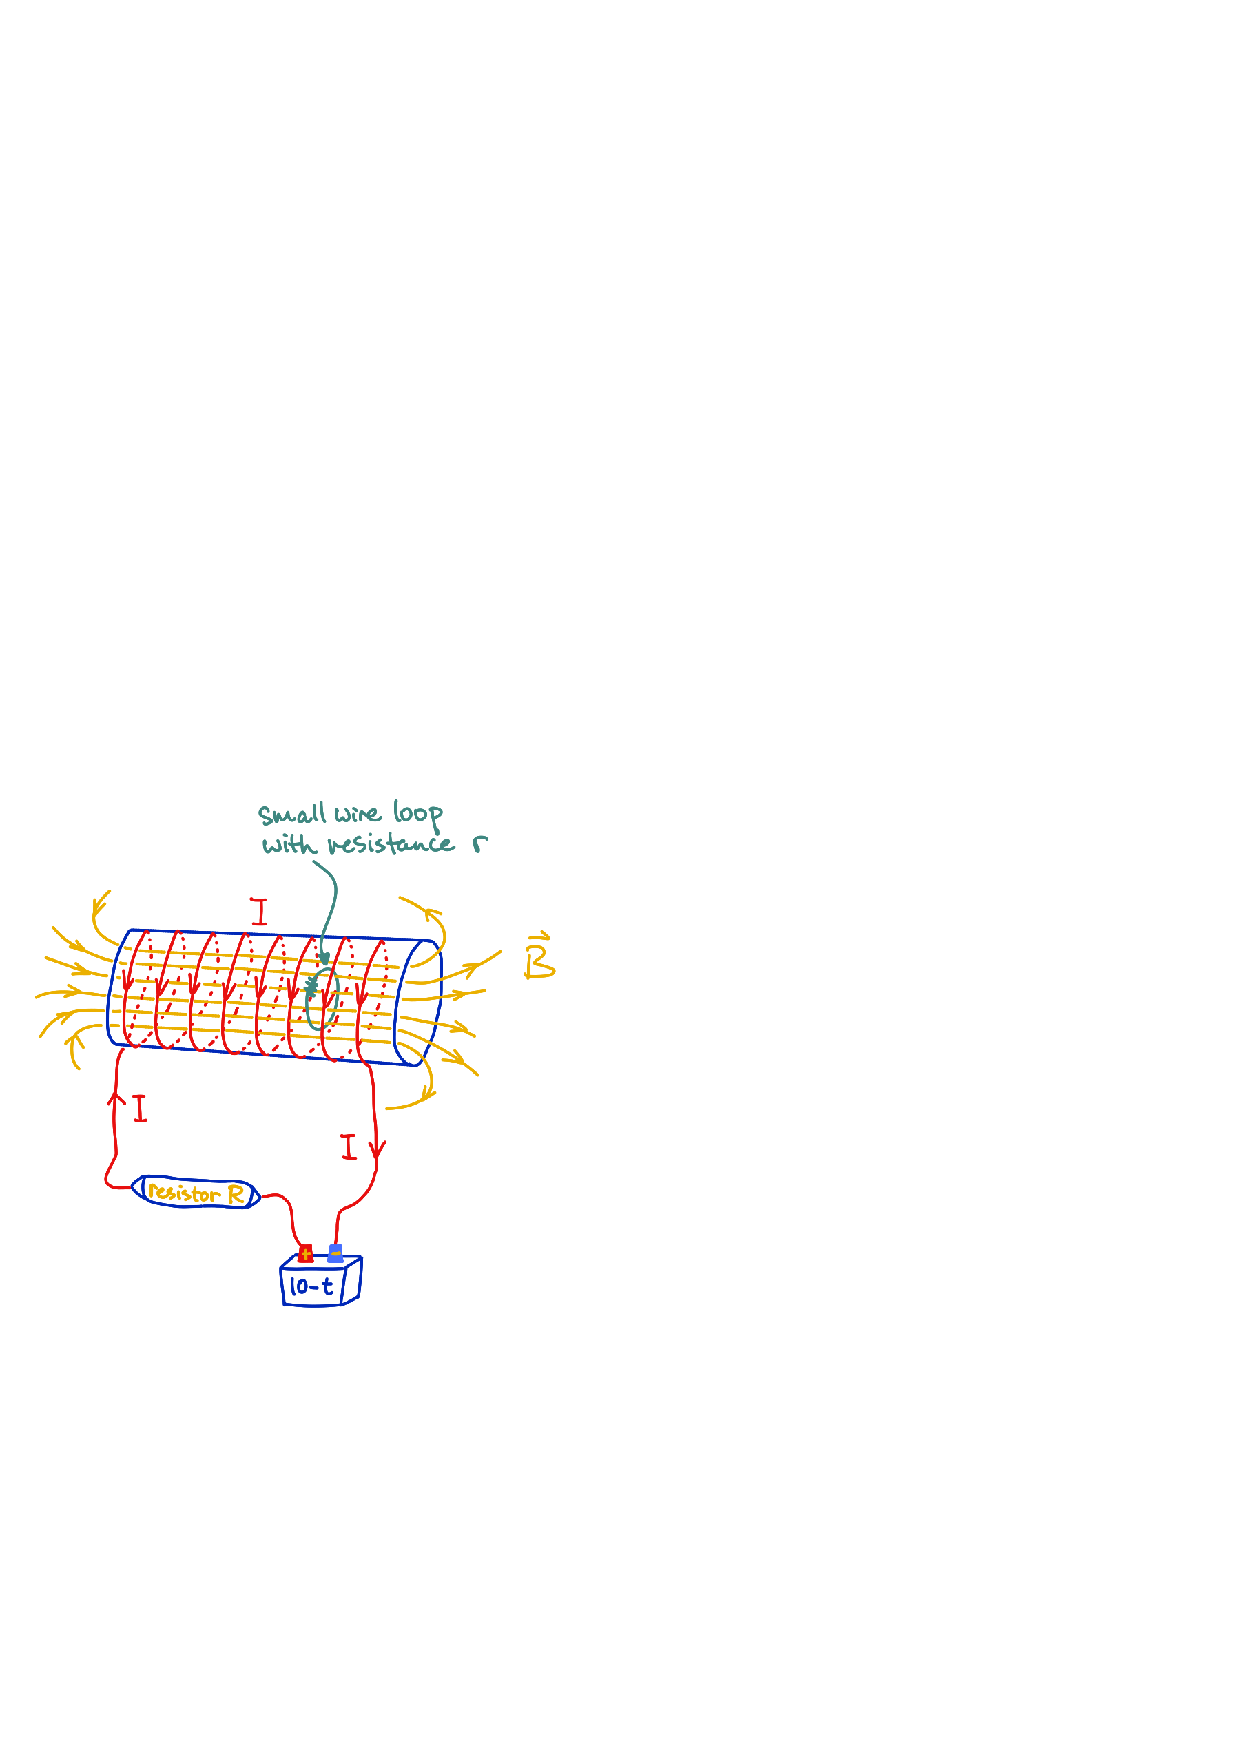
\includegraphics[scale=0.85]{solenoidInduction}
  \end{center}
\end{wrapfigure}
Jinyan is powering up a solenoid using a power source $V$ that varies in time. There is a steady current running through the solenoid, but it will change in time as Jinyan changes the power source $V$. There is a smaller wire loop inside the solenoid (drawn in indigo), with enclosed area $A$, concentric with the solenoid. The small wire loop has resistance $r$. If Jinyan dials down the voltage $V = 10-t$ as a function of time (voltage is measured in Volts), find symbolically the induced current in the small wire loop at $t = 5$\,s. \footnote{This is a simplified version of the working mechanism of transformers (not the movie). We usually see this device at some electric poles on the street. It helps step voltage up (or down) while keeping overall electric power constant.}



\newpage
\section*{Problem 1}
The magnetic field is uniform and points out of the page, so the only thing that changes is how much of the square loop has entered region $M$. Since changing magnetic flux produces an emf in the loop, we first find the immersed area, then the flux, and finally the induced emf and current.\\

\noindent\textbf{Part (a)} From the figure, the loop is a $1\,\text{m}\times 1\,\text{m}$ square. It moves to the right with speed $5\,$m/s. Therefore, after time $t$, the distance that the front edge has moved into region $M$ is $x = vt = 5t$\,. As long as the loop is still \underline{entering} the region, the immersed area is
\begin{align*}
A = (1\,\text{m})(5t\,\text{m}) = 5t\,\text{m}^2\,.
\end{align*}
This formula is valid until the whole loop has entered the region. Since the loop is $1\,$m wide, the entry process finishes when $
5t = 1$, and thus at $t = 0.2\,\text{s}$\,. Therefore,
\begin{align*}
A(t)=
\begin{cases}
5t\,\text{m}^2\,, & 0<t<0.2\,\text{s}\,,\\
1\,\text{m}^2\,, & t\ge 0.2\,\text{s}\,.
\end{cases}
\end{align*}

\noindent\textbf{Part (b)} The magnetic flux through the loop is
\begin{align*}
\Phi_B = BA\cos(\theta)\,.
\end{align*}
Here the magnetic field is perpendicular to the loop, so the angle between the loop's normal and the direction of $\vec{B}$ is $\theta=0$. Thus $\cos(\theta)=1$. Also $B=1\,$T. Therefore,
\begin{align*}
\Phi_B(t)=
\begin{cases}
5t\,\text{Wb}\,, & 0<t<0.2\,\text{s}\,,\\
1\,\text{Wb}\,, & t\ge 0.2\,\text{s}\,.
\end{cases}
\end{align*}

\noindent\textbf{Part (c)} The magnetic flux stops changing when the immersed area stops changing, that is, when the entire loop has entered region $M$. From part (a), this happens at
\begin{align*}
t = 0.2\,\text{s}\,.
\end{align*}

\noindent\textbf{Part (d)} At time $t=0.1\,$s, the loop is still entering the field region. From part (a), during this stage the immersed area is
\begin{align*}
A(t)=5t\,\text{m}^2\,.
\end{align*}
So the area is increasing at a rate of
\begin{align*}
\frac{\Delta A}{\Delta t}=5\,\text{m}^2/\text{s}\,.
\end{align*}
Since $B=1\,\text{T}$, the magnetic flux is increasing at a rate of
\begin{align*}
\frac{\Delta \Phi_B}{\Delta t}=B\,\frac{\Delta A}{\Delta t}=(1\,\text{T})(5\,\text{m}^2/\text{s})=5\,\text{Wb/s}\,.
\end{align*}
Therefore, the magnitude of the induced emf is
\begin{align*}
\varepsilon = 5\,\text{V}\,.
\end{align*}
The induced current is then
\begin{align*}
I = \frac{\varepsilon}{R} = 1\,\text{A}\,.
\end{align*}
The direction of the current is obtained via Lenz's law: The \underline{outward magnetic flux is} \underline{increasing}, so by Lenz's law the induced current must create a magnetic field pointing \underline{into the page to oppose that increase}. By the right-hand rule, that means the current runs \underline{clockwise} to produce a field into the page.\\

\noindent\textbf{Part (e)} At time $t=19^{57}\,$s, the situation is different from part (d). By then, the entire loop has long been inside the uniform field region, so the flux is constant. Therefore, $\Delta \Phi_{B}/\Delta t = 0\,$Wb$/$s, and thus $\varepsilon = 0\,\text{V}$ with $I=0\,\text{A}$\,.

\section*{Problem 2}
This problem combines several ideas together. First, the battery and resistor $R$ determine the current in the solenoid. Second, that current determines the magnetic field inside the solenoid. Third, if that magnetic field changes in time, the magnetic flux through the indigo small loop changes, which induces an emf and hence an induced current in the small loop.\\

Here I draw the big circuit (drawn in red in the cartoon).
\begin{center}
\begin{circuitikz}[scale=0.95, transform shape]
\draw
(0,0) to[battery1] (0,3)
      -- (1.2,3) to[L] (4.2,3)
      to[R] (4.2,0) -- (0,0);
\node at (-0.8,1.5) {$V$};
\node at (2.7,3.7) {$\text{solenoid}$};
\node at (4.8,1.5) {$R$};
\end{circuitikz}
\end{center}

\noindent For the big circuit containing the solenoid, the solenoid is just a chunk of twisted wire, so there is no resistance in it. Thus we use Ohm's law to find the current in the circuit, which is also the current that runs through the solenoid,
\begin{align*}
I_{\text{solenoid}} = \frac{V}{R} = \frac{10-t}{R}\,.
\end{align*}
Inside a long solenoid, the magnetic field is
\begin{align*}
B = \frac{\mu_0 N I_{\text{solenoid}}}{L}
= \frac{\mu_0 N (10-t)}{LR}\,.
\end{align*}
So the magnetic flux through the small loop of area $A$ is
\begin{align*}
\Phi_B = BA = \frac{\mu_0 N A(10-t)}{LR}\,.
\end{align*}
Now we ask how fast this flux is changing. Since $V=10-t$, the voltage drops by $1$ Volt every second. Therefore the current in the solenoid drops by
$1/R$ Amps per second, so the magnetic field drops by $\mu_0 N/(LR)$
each second, and the magnetic flux through the small loop changes by
\begin{align*}
\frac{\Delta \Phi_{B}}{\Delta t}=- \frac{\mu_0 N A}{LR}\,.
\end{align*}
Therefore the magnitude of the induced emf in the small loop is
\begin{align*}
\varepsilon_{\text{ind}} =\left| \frac{\Delta \Phi_{B}}{\Delta t}\right|=  \frac{\mu_0 N A}{LR}\,.
\end{align*}
If you know calculus, this is way easier: We only need to use the $\Phi_B$ we just calculated,
\begin{align*}
\varepsilon_{\text{ind}} = \left| 
\frac{d\Phi_{B}}{dt}
\right| = \frac{\mu_0 N A}{LR}\,.
\end{align*}
Since the small loop has resistance $r$, the induced current in that loop is
\begin{align*}
I_{\text{ind}} = \frac{\varepsilon_{\text{ind}}}{r}
= \frac{\mu_0 N A}{LRr}\,.
\end{align*}
This is the symbolic answer at $t=5\,$s. In fact, because the source voltage is decreasing linearly in time, the induced current has the same magnitude at every time until the voltage stops changing, not just at $t=5\,$s.\\

For the direction, Lenz's law says that the induced current must try to \underline{oppose the} \underline{decrease} in magnetic flux. So the induced current in the small loop runs in whatever direction creates a magnetic field in the \underline{same direction} as the original solenoid field inside the loop.\\


\vfill
\begin{center}

\includegraphics[scale=0.42]{DSC06903.JPG}\\
\hfill\break
Sunrise at Madison, Wisconsin. Pictured by Jinyan in March 2024.\\
It serves as the background picture on my iPhone-13 and my laptop :)
\end{center}


\end{document}
